\documentclass[tikz,border=8pt]{standalone}
\usepackage{amsmath,amssymb}
\usepackage{tikz}
\usetikzlibrary{arrows.meta,calc}

\begin{document}
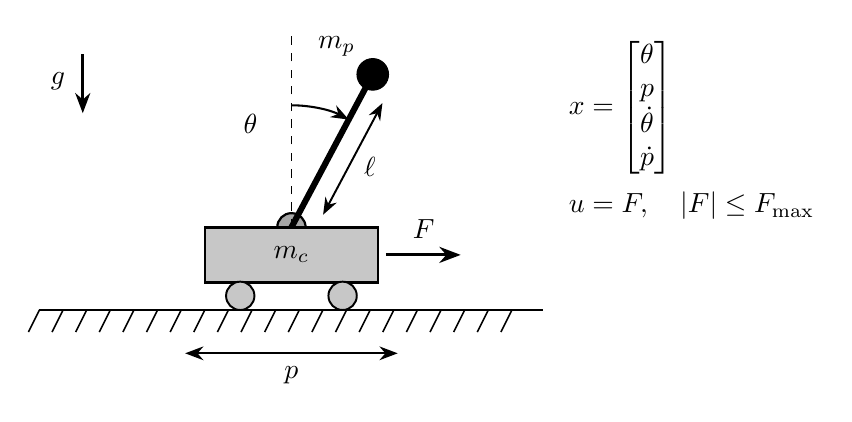
\begin{tikzpicture}[
  >=Stealth,
  font=\normalsize
]
  % ground
  \draw[line width=0.95pt] (-3.2,0) -- (3.2,0);
  \foreach \x in {-3.2,-2.9,...,3.1}
    \draw[line width=0.55pt] (\x,0) -- ++(-0.14,-0.28);

  % cart
  \coordinate (Pivot) at (0,1.05);
  \filldraw[fill=black!22, draw=black, line width=0.9pt]
    (-1.1,0.35) rectangle (1.1,1.05);
  \node at (0,0.70) {$m_c$};
  \filldraw[fill=black!22, draw=black, line width=0.7pt] (-0.65,0.18) circle (0.18);
  \filldraw[fill=black!22, draw=black, line width=0.7pt] (0.65,0.18) circle (0.18);
  \draw[line width=0.8pt, fill=black!35] (-0.18,1.05) arc (180:0:0.18) -- cycle;

  % pole (tilt from upright)
  \def\poleang{-28}
  \def\polelen{2.20}
  \coordinate (Tip) at ($(Pivot)+({90+\poleang}:\polelen)$);
  \draw[line width=2.2pt] (Pivot) -- (Tip);
  \filldraw[fill=black, draw=black] (Tip) circle (0.20);
  \node[anchor=south east] at ($(Tip)+(-0.10,0.10)$) {$m_p$};

  % upright + angle
  \draw[dashed, line width=0.5pt] (Pivot) -- ($(Pivot)+(0,2.45)$);
  \draw[->, line width=0.75pt]
    ($(Pivot)+(0,1.55)$) arc (90:{90+\poleang}:1.55);
  \node at ($(Pivot)+(-0.52,1.32)$) {$\theta$};

  % length dimension along pole
  \draw[<->, line width=0.7pt]
    ($(Pivot)!0.15!(Tip)+(\poleang:0.28)$) --
    ($(Pivot)!0.88!(Tip)+(\poleang:0.28)$);
  \node at ($(Pivot)!0.52!(Tip)+(\poleang:0.52)$) {$\ell$};

  % force
  \draw[->, line width=1.05pt] (1.2,0.70) -- (2.15,0.70);
  \node[anchor=south] at (1.68,0.78) {$F$};

  % position
  \draw[<->, line width=0.8pt] (-1.35,-0.55) -- (1.35,-0.55);
  \node[anchor=north] at (0,-0.60) {$p$};

  % gravity
  \draw[->, line width=0.95pt] (-2.65,3.25) -- (-2.65,2.50);
  \node[anchor=east] at (-2.75,2.90) {$g$};

  % equations
  \node[anchor=north west, align=left] at (3.4,3.55) {%
    $\displaystyle x=\begin{bmatrix}\theta\\ p\\ \dot{\theta}\\ \dot{p}\end{bmatrix}$\\[5pt]
    $\displaystyle u=F,\quad |F|\le F_{\max}$%
  };
\end{tikzpicture}
\end{document}
